\chapter{The chain of custody}\label{ch:chain}

\section{What the chain is}

The Cellular Performance Gauge is a chain of stages that takes a specimen's raw array files and returns a reading on the one gauge of
Chapter~\ref{ch:gauge}. Chain v4, the first commissioned chain, carries five instruments, each commissioned for its own scope: Met-A on isolated neutrophils (EPIC v1, 2026-10-09), the C-score on whole blood (2026-10-15), IAM-Atlas v2.1 for three cell references and the colon and lung tissue tests (2026-10-16), the IAM-Deconvolver for the shares of neutrophils, monocytes, CD4 and CD8 T cells (2026-10-17), and IAM-A on healthy CD8 T cells, read by whole-genome sequencing against each sample's own reference (2026-10-17). A reading outside an instrument's tested scope is printed with a plain note saying so. It is a research instrument, not a diagnostic test; its scope grows one cell type and one specimen at a time, each after it passes its own sealed test. The
procedure is the SOP and the operations manual.
Where a document and the code differ, the code is what runs. This chapter walks through the stages (Figure~\ref{fig:chain}).

Table~\ref{tab:p4_gates} lists the line each stage applies; the values and the files they are read from are in the SOP.

\begin{table}[htbp]\centering\small
\caption{The lines chain v4 applies, stage by stage. Values are read from frozen files (FROZEN\_INPUTS\_v4.json); platform, Stage~M and Stage~T rules as stated in this chapter. \calibrated}\label{tab:p4_gates}
\begin{tabular}{@{}lp{0.5\textwidth}p{0.3\textwidth}@{}}\toprule
stage & line & source \\\midrule
Stage 0 & call rate: proceed; flagged; quarantine & SOP \\
Stage 0 & bisulfite conversion at least 0.80; hybridization spread at least 2.0; extension balance 0.2--5.0 & 337 healthy arrays, 3 laboratories \\
platform & EPIC v1 only & SOP \\
Stage A & enough of the composition markers measured & SOP \\
Stage M & a neutrophil share above 0; at least 90\,\% of the identity sites measured & SOP \\
Stage MC & blocks of 10 sites; enough blocks; baseline 1.0103; band 0.877--1.152, read one-sided & SOP \\
Stage T & median tare against same-run references & SOP \\
Stage D21 & IAM-Atlas v2.1 tables; the six-cell blood panel & FROZEN\_INPUTS\_v4 \\
Stage Q2 & enough qualifying molecules; the sample-shape check; self-reference line v1; band v1 0.779--1.055 & FROZEN\_INPUTS\_v4 \\
Stage SKY & C-score departures on HEALPix, NSIDE 128, nested order; nothing scored & FROZEN\_INPUTS\_v4 \\
\bottomrule
\end{tabular}
\end{table}

\begin{figure}[htbp]\centering
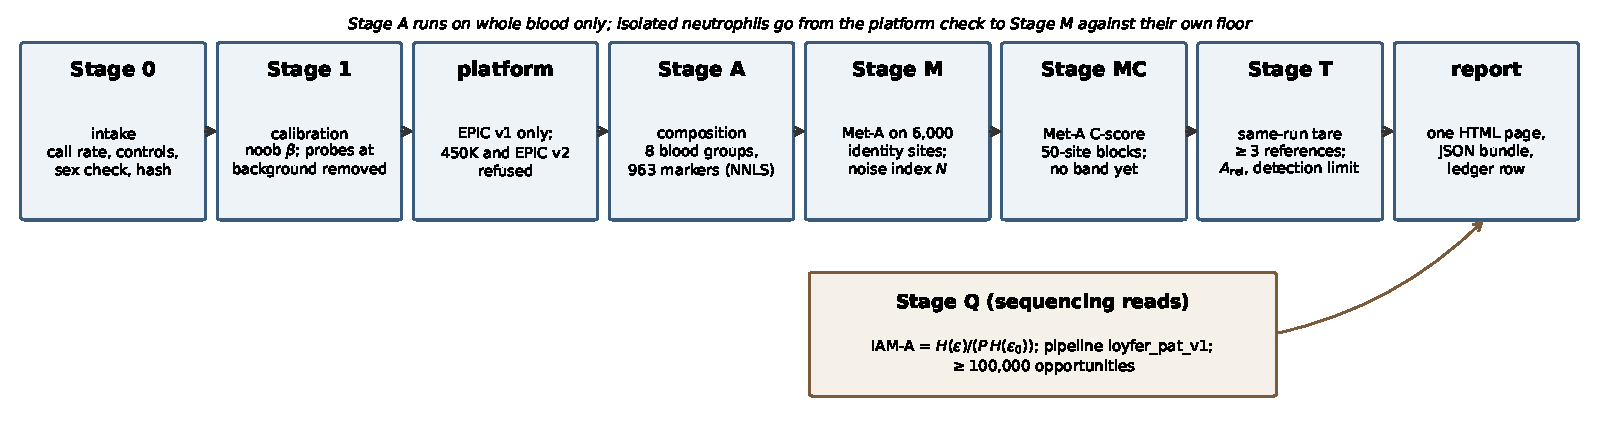
\includegraphics[width=\textwidth]{figures/part6/fig_chain_v3_flow.pdf}
\caption{Chain v3, from intake to report. Stage~A runs on whole blood only. Stage~Q reads sequencing input. Drawn from the stage rules in the code.}
\label{fig:chain}
\end{figure}

\section{Stage 0: intake}

The IDAT pair is opened and the array's own numbers are read: manifest, integrity hash, control probes, per-probe detection, call rate and sex check.
Below the lower call-rate line the specimen is quarantined and no reading is written; between the lines it proceeds with a flag. A sex mismatch, a failed
integrity check or a deferred detection or call-rate check also quarantines (Chapter~\ref{ch:instrument}). A cleartext identifier is hashed before the
engine sees it. Input that arrives as $\beta$ values without the raw files can be read, but no intake runs on it: the v3 bundle carries no intake record,
and the report prints intake as not run.

\section{Stage 1: calibration}

Noob background and dye-bias correction and probe-type normalization, per array, produce $\beta$ at every probe. Probes indistinguishable from background are
removed before any later stage sees a $\beta$. Stage~1 returns, beside $\beta$, the array's detection numbers and control intensities.

\section{Platform check}

The chain reads EPIC v1 only. A specimen whose array type, probe names or probe count say 450K or EPIC v2 is refused with one sentence, because no frozen
neutrophil floor exists for that platform.

\section{Stage A: composition (whole blood)}

Eight blood groups are solved by non-negative least squares on markers, none of them a neutrophil identity site (Chapter~\ref{ch:separation}). Too few
measured markers: no composition and no reading. Isolated neutrophils skip this stage.

\section{Stage M: Met-A}

\begin{itemize}
\item \textbf{Isolated neutrophils:} the mean $H(\beta)$ over the identity sites divided by the floor, 0.330263 bits (Eq.~\eqref{eq:meta}).
\item \textbf{Whole blood:} read when the neutrophil fraction is above the read line; the mean $H(\beta)$ over the sites divided by the mean $H(e)$ of the specimen's
      own healthy expectation (Eq.~\eqref{eq:metawb}). Below the line the fraction is printed and $A$ is withheld.
\end{itemize}
Either way enough of the sites must be measured. Stage~M also records the noise index $N$, the shift a 1~\% loss of the neutrophil pattern would cause in
this specimen, and the methylated sites' mean $\beta$ with a flag when it is below one half, past the entropy ceiling.

\section{Stage MC: the Met-A C-score}

The residual map over the identity sites, in genome order, is reduced to the C-score: the variance of 50-site block means, times 50, over the variance of the sites,
divided by the healthy baseline 1.1104 (Chapter~\ref{ch:cscore}). It is printed with every reading, with no band. The IAM-A C-score is defined and not yet built. \openprob

\section{Stage T: the tare}

The reading is divided by the median of healthy references of the same specimen type run the same way, on the same slide, else in the same batch.
The result is $A_{\rm rel}$, and the gauge state is printed from $A_{\rm rel}$ only: \emph{Normal} (0.95--1.05), \emph{above Normal} or \emph{below Normal}. Every
tared reading carries its detection limit: twice the references' spread over the shift per 1~\% loss, the smallest loss of the neutrophil pattern this specimen
could have shown.

The noise index $N$, the mean $H(\beta)$ over the sites that every purified blood group holds fixed, is measured on every array and gates the gauge
state: outside the range of the purified reference arrays the state is withheld.
There is no fitted correction for $N$. \calibrated{} A slide tare from fully methylated and fully unmethylated control DNA run on every slide is the planned tare.
\openprob{} (until a laboratory runs it)

Without references, whole blood is printed as \emph{untared}, with no state and no gauge position. Isolated neutrophils without references keep their healthy-reference
state inside the untared label (\emph{untared (healthy-reference state: \dots)}) and are drawn on the gauge against their healthy reference, labeled untared.

The operating procedure is in the operations manual.

% COMMISSIONING-RETURN fig:p4_detlimit: figure taken out 2026-10-03 (plotted development values from the removed fitted tare). Put back, redrawn from the commissioned chain; see development/COMMISSIONING_RETURNS.md.


\section{Stage Q2: IAM-A against the sample's own reference}

Single-molecule input (a read-level \texttt{.pat} file or an aligned whole-genome bisulfite BAM) passes the intake checks of Stage Q0,
is counted once for its held error and its loose share, passes the sample-shape check, and is read as IAM-A, Eq.~\eqref{eq:iama}, on
band v1. Commissioned 2026-10-17 on healthy blood CD8 T cells; every other cell type is read and printed with the note that it has not yet been tested with this instrument. The earlier position
reading (Stage Q, Eq.~\eqref{eq:iamapos}) runs only behind a development flag.

\section{Chain v4: the commissioned instruments in one run}

Chain v4 (2026-10-17) keeps every stage of chain v3 and adds three. After the array reading, the IAM-Deconvolver reads the cell shares
against IAM-Atlas v2.1 (commissioned for neutrophils, monocytes, CD4 and CD8 T cells), and the C-score's departures are drawn on a
HEALPix sphere in nested order, where neighboring sites fill compact patches; the drawing is a picture of the reading and nothing is
scored from it. Sequencing input goes to Stage Q2 above. One command, \texttt{release\_check\_v4.py}, runs every check of the chain
from a fresh copy of the public repository. Where this part says ``chain v3'', the stage it describes is carried unchanged into v4.

% SEX-SECTION:BEGIN
\paragraph{Sex and the X chromosome.} A woman has two X chromosomes and silences one in every cell by methylating it (X inactivation). At the switch sites of hundreds of X genes a man's single X reads near 0 and a woman's two copies average about 0.5. The Y exists only in men. A comparison between people of different sex can therefore light up the X without any disease. Each instrument handles this as follows (numbers computed from the chain's own files by \texttt{CANON/sex\_chromosomes.py}):
\begin{description}
\item[Stage 0, intake] Predicts the array's sex from its X and Y probe brightness (step 0.8: female when log2 Y minus log2 X is below -2.0). When a sex is declared and the array disagrees, the array is stopped and the reason printed: a swapped sample is caught before any reading.
\item[Met-A] 6,000 neutrophil identity sites: 32 on the X, 0 on the Y. They were chosen where the six purified reference arrays, one of them a woman's, agree. Group-A's sealed test read 75 women and 188 men the same after the tare (-0.36 \%, 1.2 standard errors).
\item[C-Score] The same 6,000 sites (32 on the X, 0 on the Y), in genome order; it reads how departures cluster, read against the same healthy reference.
\item[Noise index] 48,528 sites, 95 on the X and 15 on the Y. Even if every one of them read at maximum noise, the index could move by at most 0.0023 bits (0.23 \% of its 1-bit scale).
\item[Stage A, the blood mix] 963 markers, 0 on the X or Y.
\item[IAM-Deconvolver] 600 markers, 0 on the X, 0 on the Y.
\item[IAM-A] Each sample is read against its own predicted error, so no other person, of either sex, enters its reading. Aligned files (BAM) are counted on chromosomes 1 to 22 only. From a .pat file the loose share is counted on chromosomes 1 to 22, and the held error on every chromosome the file holds (the route IAM-A was commissioned on; a recount with the X and Y left out is on the to-do list, Decoder finding F37).
\item[Group-A] Compares groups run in the same series; its sealed bar 2 is a women-against-men null (above).
\item[IAM-Atlas v2.1 and the globes] 813,951 atlas sites, 14,759 on the X and 3 on the Y. The atlas's donors are women and men, so it is 2.5 to 3.6 times less sure on the X and Y than elsewhere (the noise globe shows it). Every change count on a globe is also given on the X and Y, the page prints the sex Stage 0 read, and a tumor against its own normal tissue (same person, same sex) is counted with and without the X and Y: in a tumor an X change can be real biology.
\end{description}
% SEX-SECTION:END

\section{What the chain withholds}

Every bundle lists what the build does not print: any line beyond Normal, because breach and the cancer region are not yet measured on this scale. A cell type or specimen outside an instrument's tested scope is read and printed with that note. The whole-array sky, serial mode and the out-of-span map are not part of chain v4. \openprob

\section{The record of a run}

Each run writes one HTML page, a JSON bundle with every stage's output and the versions of the floor and reference files, and one row appended to an evidence
ledger (Chapter~\ref{ch:report}). Each run takes its number from the ledger. The v3 bundle does not yet record the chain's commit or a checksum of each
frozen file it read, and the v3 procedure and operations manual are written by hand, not generated from the code. \openprob
